Beginning of Introduction.\\~\\
You can cite with \cite{nadeau_2019}.

%Make sure to include [H] to place the figure in the text
\begin{figure}[H]
    \centering
    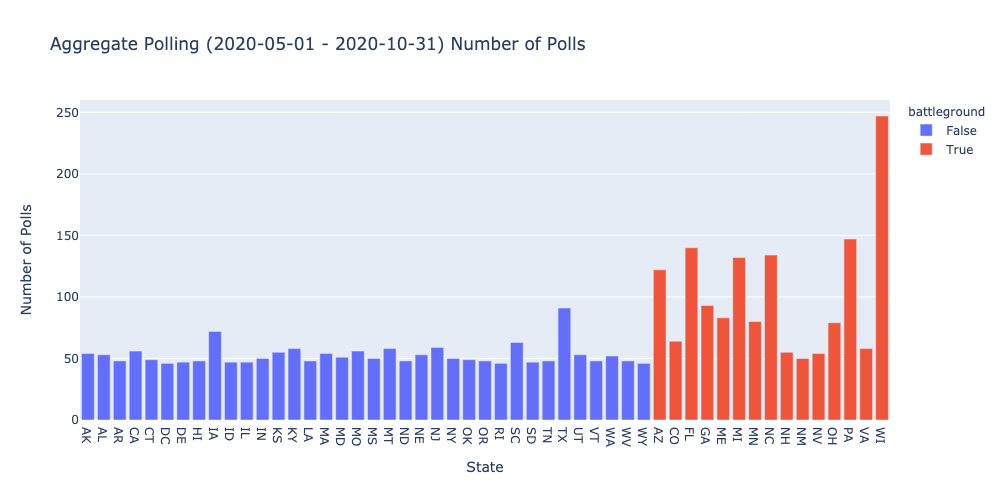
\includegraphics[height=20em]{figures/aggregate_polling_2020-05-01_-_2020-10-31_number_of_polls.png}
    \label{fig:aggregate_polling_2020-05-01_-_2020-10-31_number_of_polls}
\end{figure}

\begin{table}[H]
\begin{table}
\centering
\caption{Aggregate Polling (2020-05-01 - 2020-10-31) Number of Polls}
\begin{tabular}{lr}
\toprule
 battleground &        mean \\
\midrule
        False &   52.666667 \\
         True &  102.533333 \\
\bottomrule
\end{tabular}
\end{table}

    \label{tab:aggregate_polling_2020-05-01_-_2020-10-31_number_of_polls}
\end{table}

As shown in \ref{tab:aggregate_polling_2020-05-01_-_2020-10-31_number_of_polls}, we see that there is more polling in battleground states than non-battleground states.\\

\begin{figure}[H]
    \centering
    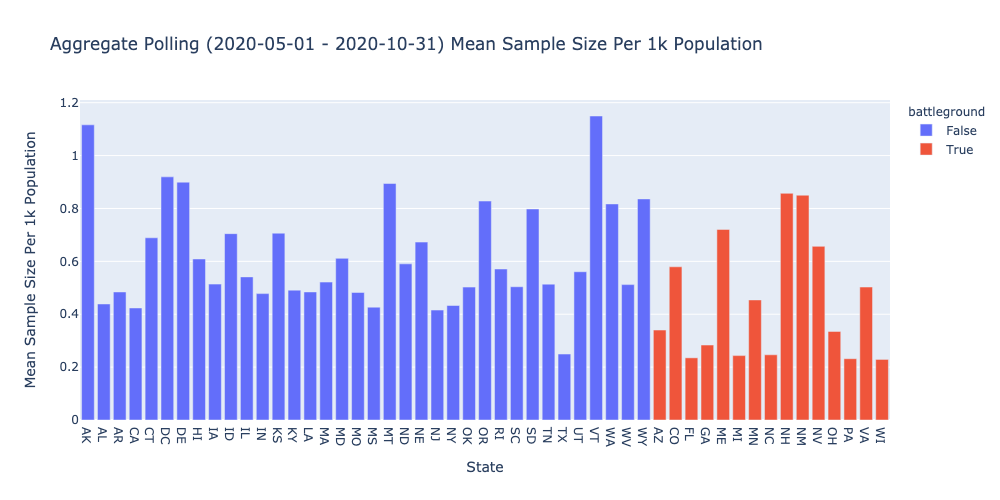
\includegraphics[height=20em]{figures/aggregate_polling_2020-05-01_-_2020-10-31_mean_sample_size_per_1k_population.png}
    \label{fig:aggregate_polling_2020-05-01_-_2020-10-31_mean_sample_size_per_1k_population}
\end{figure}

\begin{table}[H]
\begin{table}
\centering
\caption{Aggregate Polling (2020-05-01 - 2020-10-31) Mean Sample Size Per 1k Population}
\begin{tabular}{lr}
\toprule
 battleground &      mean \\
\midrule
        False &  0.621980 \\
         True &  0.451055 \\
\bottomrule
\end{tabular}
\end{table}

    \label{tab:aggregate_polling_2020-05-01_-_2020-10-31_mean_sample_size_per_1k_population}
\end{table}

